\documentclass[a4paper]{article}

\usepackage[english]{babel}
\usepackage{amsmath}
\usepackage{color}
\usepackage{amssymb}
\usepackage{dsfont}
\usepackage{multicol}
%\usepackage[lofdepth,lotdepth]{subfig}  This gives errors when used together with "subcaption", which is needed to create subfigures.
\usepackage{graphicx}
\usepackage{listings}
\usepackage[hyphens]{url}
\usepackage{pgf, tikz}
\usetikzlibrary{arrows, automata}
\usepackage{titling}
\usepackage{varwidth}
\usepackage{hyperref}
\usepackage{color} %red, green, blue, yellow, cyan, magenta, black, white
\definecolor{mygreen}{RGB}{28,172,0} % color values Red, Green, Blue
\definecolor{mylilas}{RGB}{170,55,241}
\setlength\parindent{0pt}
\usepackage{float}
\usepackage{subcaption}
\usepackage{polynom}
\usepackage{physics}
\newcommand\tab[1][1cm]{\hspace*{#1}}


\newcommand\independent{\protect\mathpalette{\protect\independenT}{\perp}}
\def\independenT#1#2{\mathrel{\rlap{$#1#2$}\mkern2mu{#1#2}}}

\usepackage{geometry}
 \geometry{
 a4paper,
 total={165mm,257mm},
 left=20mm,
 top=20mm,
 }

\definecolor{codegreen}{rgb}{0,0.6,0}
\definecolor{codegray}{rgb}{0.5,0.5,0.5}
\definecolor{codepurple}{rgb}{0.58,0,0.82}
\definecolor{backcolour}{rgb}{0.95,0.95,0.92}

\lstdefinestyle{mystyle}{
    backgroundcolor=\color{backcolour},   
    commentstyle=\color{codegreen},
    keywordstyle=\color{magenta},
    numberstyle=\tiny\color{codegray},
    stringstyle=\color{codepurple},
    basicstyle=\footnotesize,
    breakatwhitespace=false,         
    breaklines=true,                 
    captionpos=b,                    
    keepspaces=true,                 
    numbers=left,                    
    numbersep=5pt,                  
    showspaces=false,                
    showstringspaces=false,
    showtabs=false,                  
    tabsize=2
}
 
\lstset{style=mystyle}


\DeclareMathOperator*{\argmax}{arg\,max}
\DeclareMathOperator*{\argmin}{arg\,min}

\title{Statistical Machine Learning 2018\\Assignment 4\\Deadline: 11th of January 2019}
\author{
  Christoph Schmidl\\ s4226887\\      \texttt{c.schmidl@student.ru.nl}
  \and
  Mark Beijer\\ s4354834\\     \texttt{mbeijer@science.ru.nl}
}
\date{\today}

\begin{document}
\maketitle


\section*{Exercise 1 - Logistic regression (weight 5)}

\textbf{Part 1 - The IRLS algorithm}\\




\textbf{Part 2 - Two-class classification using logistic regression}\\




\section*{Exercise 2 - Neural network regression (weight 5)}

We train a neural network using backpropagation, to learn to mimic a 2D multimodal probability density. First, we implement the network and test its regression capabilities on a standard Gaussian; then we train it on the real data set. Visualization of the network output plays an important role in monitoring the progress.

\subsection*{2.1}

Create a plot of an isotropic 2D Gaussian $y = 3 \cdot \mathcal{N}(\textbf{0}|\frac{2}{5}\textbf{I}_2)$ centered at the origin using the \texttt{meshgrid()}, \texttt{mvnpdf()} and \texttt{surf()} functions. Sample the density at 0.1 intervals over the range $[-2,2] \times [-2,2]$ and store the data in colum vector variables $\textbf{X}$ (2D) and $\textbf{Y}$ (1D).\\

\textbf{Answer:}\\







\subsection*{2.2}

Implement a 2-layer neural network with $D = 2$ input nodes, $K = 1$ output nodes and $M$ hidden nodes in the intermediate layer that can be trained using a sequential error backpropagation procedure, as described in Bishop §5.3. Use $tanh(\cdot)$ activation functions for the hidden nodes and a linear activation function (regression) for the output node. Introduce appropriate weights and biases, and set the learning rate parameter $\eta = 0.1$. Initialize the weights to random values in the interval $[-0.5,0.5]$. Plot a 2D graph of the initial output of the network over the same $[-2,2] \times [-2,2]$ grid as the Gaussian (again using \texttt{surf()}).\\

\textbf{Answer:}\\









\subsection*{2.3}

Train the network for $M = 8$ hidden nodes on the previously stored $\textbf{X}$ and $\textbf{Y}$ values (the $\{ x_1, x_2 \}$ input coordinates and corresponding output probability density $y$), by repeatedly looping over all datapoints and updating the weights in the network after each point. Repeat for at least 500 complete training cycles and monitor the progress of the training by plotting the output of the network over the $\textbf{X}$ grid after each full cycle. Verify the output starts to resemble the Gaussian density after some 200 cycles (all be it with lots of 'wobbles').\\


\textbf{Answer:}\\







\subsection*{2.4}

Permute the $\textbf{X}$ and $\textbf{Y}$ arrays to a random order using the \texttt{randperm()} function, keeping corresponding $x$ and $y$ together. Repeat the network training session using this randomized data set. Verify that convergence is now much quicker. Can you understand why? Try out the effect of different numbers of hidden nodes, different initial weights and different learning rates on speed and quality of the network training. Explain your results.

\begin{figure}[H]
\center
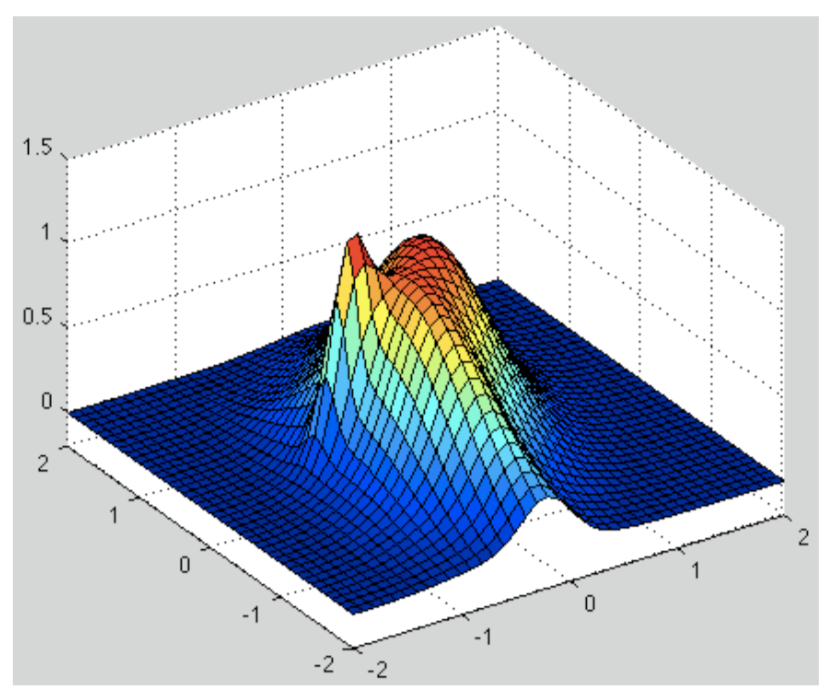
\includegraphics[width=0.4\textwidth]{Images/multi-modal.png}
\caption{Multi-modal probability density}
\label{Fig:multi-modal}
\end{figure}



After these preliminaries we are now going to train the network on the real data set.\\
Load the data using\\


\hspace{1cm} \texttt{data = load('a017\_NNpdfGaussMix.txt', '-ASCII');}

\hspace{1cm} \texttt{X = data(:,1:2); Y = data(:,3);}\\

\textbf{Answer:}\\






\subsection*{2.5}

Create a $2D$-plot of the target probability density function. Notice that the data is in the correct sequence to use in \texttt{surf()}.\\

\textbf{Answer:}\\








\subsection*{2.6}

Train the network on this data set. Use at least 40 hidden nodes and a learning rate parameter no higher than $\eta = 0.01$. Make sure the input data is properly randomized. Run the training phase for at least 2000 complete cycles and follow the progress by plotting the updated network output after every 20 full cycles. How does the final output of the network compare to the target distribution in the data? Explain. How could you improve the neural network in terms of speed of convergence and/or quality of the approximation?



\section*{Exercise 3 - Gaussian processes (weight 5)}


\textbf{Part 1 - Sampling from Gaussian stochastic processes}\\




\textbf{Part 2 - Gaussian processes for regression}\\



\section*{Exercise 4 - EM and doping (weight 5)}





\subsection*{3.2d}



\subsection*{3.2e}



\end{document}
